\documentclass[margin=0.1cm]{standalone}
\usepackage{ tikz }
\usepackage{ xparse }
\usepackage{../../../macros}

\begin{document}
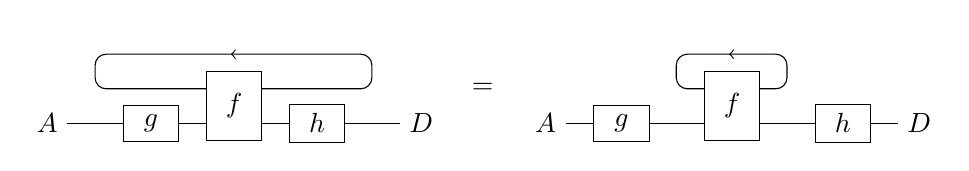
\begin{tikzpicture}[yscale=-1,x=1em,y=1.25em]
        
    \node at (0,-2.5) {$\null$};

    \node [anchor=east] at (0,0) {$A$};
    \node [anchor=west] at (12,0) {$D$};

    \draw (0,0) -- (2,0);
    \node[draw, minimum height = 1em, minimum width = 2em, anchor = west, fill=white] at (2,0){$g$};
    \draw (4,0) -- (5,0);
    \node[draw, minimum height = 2.5em, minimum width = 2em, anchor = west, fill=white] at (5,-0.5){$f$};
    \draw (7,0) -- (8,0);
    \node[draw, minimum height = 1em, minimum width = 2em, anchor = west, fill=white] at (8,0){$h$};
    \draw (10,0) -- (12,0);
    \draw [->, rounded corners] (7,-1) -- (11,-1) -- (11,-2) -- (5.9,-2);
    \draw [rounded corners] (5.9,-2) -- (1,-2) -- (1,-1) -- (5,-1);

    \node at (15,-1) {$=$};

    \node [anchor=east] at (18,0) {$A$};
    \node [anchor=west] at (30,0) {$D$};

    \draw (18,0) -- (19,0);
    \node[draw, minimum height = 1em, minimum width = 2em, anchor = west, fill=white] at (19,0){$g$};
    \draw (21,0) -- (23,0);
    \node[draw, minimum height = 2.5em, minimum width = 2em, anchor = west, fill=white] at (23,-0.5){$f$};
    \draw (25,0) -- (27,0);
    \node[draw, minimum height = 1em, minimum width = 2em, anchor = west, fill=white] at (27,0){$h$};
    \draw (29,0) -- (30,0);
    \draw [->, rounded corners] (25,-1) -- (26,-1) -- (26,-2) -- (23.9,-2);
    \draw [rounded corners] (23.9,-2) -- (22,-2) -- (22,-1) -- (23,-1);

\end{tikzpicture}
\end{document}